\documentclass[10pt,journal,a4paper]{IEEEtran}

% ── Encodage et langue ───────────────────────────────────────────
\usepackage[utf8]{inputenc}
\usepackage[T1]{fontenc}
\usepackage[french]{babel}

% ── Maths, figures, tableaux ─────────────────────────────────────
\usepackage{amsmath,amssymb}
\usepackage{graphicx}
\usepackage{booktabs}
\usepackage{url}
\usepackage[hidelinks]{hyperref}

\begin{document}

% ─────────────────────────────────────────────────────────────────
\title{HTmiR~: reconnaissance automatique de l'écriture manuscrite pour
le français médiéval --- vers les carnets spéculaires de Léonard de Vinci}

\author{%
\IEEEauthorblockN{Abdessamad Touzani, Emmanuel (morningstar-manu)}\\
\IEEEauthorblockA{HETIC --- Master Recherche, Module Computer Vision, 2026\\
\texttt{abdessamadtz6@gmail.com}}%
}

\maketitle

% ─────────────────────────────────────────────────────────────────
\begin{abstract}
La reconnaissance automatique de l'écriture manuscrite (\textit{Handwritten
Text Recognition}, HTR) appliquée aux manuscrits médiévaux reste un défi en
raison de la diversité des mains, des abréviations et de la rareté des données
annotées. Notre objectif à long terme est la transcription des carnets en
\emph{écriture spéculaire} de Léonard de Vinci. Faute de vérité terrain
disponible pour ces manuscrits, nous construisons et validons d'abord un
pipeline HTR reproductible sur le \emph{français médiéval du
XIII\textsuperscript{e} siècle}, à partir du corpus CATMuS Medieval. Nous
fine-tunons le modèle Kraken \textit{CATMuS Medieval} sur près de 21\,000 lignes
filtrées et obtenons un taux d'erreur caractère (CER) de validation d'environ
\textbf{4,5\,\%}, sous notre cible de 8\,\%. Cet article décrit la collecte des
données, la méthode de fine-tuning, les résultats, et les perspectives
d'application à l'écriture de Léonard de Vinci.
\end{abstract}

\begin{IEEEkeywords}
HTR, manuscrits médiévaux, Kraken, CATMuS, transfert d'apprentissage,
français ancien, Léonard de Vinci, écriture spéculaire.
\end{IEEEkeywords}

% ─────────────────────────────────────────────────────────────────
\section{Introduction}
\IEEEPARstart{L}{éonard} de Vinci (1452--1519) a rédigé la quasi-totalité de
ses milliers de pages de carnets en \emph{écriture spéculaire} (écriture en
miroir~: de droite à gauche, lettres inversées). Ces manuscrits, en italien
toscan du Quattrocento, constituent un patrimoine scientifique majeur mais
difficilement exploitable~: leur transcription manuelle complète représenterait
des milliers d'heures de travail expert.

L'ambition initiale de ce projet était d'entraîner un modèle HTR capable de lire
directement cette écriture spéculaire. Une contrainte fondamentale est cependant
apparue~: \textbf{il n'existe pas de vérité terrain} (paires image/transcription
alignées) publiquement disponible pour les manuscrits de Léonard de Vinci. Or le
fine-tuning supervisé d'un modèle HTR exige précisément de telles paires.

Nous adoptons donc une démarche \emph{progressive et transférable}~: plutôt que
d'annoter manuellement des dizaines de pages de Vinci (hors de portée dans le
temps imparti), nous construisons et validons un pipeline HTR complet sur un
corpus médiéval richement annoté --- le français du XIII\textsuperscript{e}
siècle issu de CATMuS Medieval --- en écriture gothique \textit{textualis}.
L'écriture gothique partage avec celle de Vinci la densité, les abréviations et
les ligatures qui font la difficulté du HTR ancien. Le pipeline ainsi éprouvé
constitue la base réutilisable pour une future campagne d'annotation et de
fine-tuning sur les carnets de Léonard de Vinci.

\textbf{Contributions.} (i)~Un pipeline reproductible de collecte et de
préparation de données HTR depuis CATMuS Medieval~; (ii)~le fine-tuning d'un
modèle Kraken atteignant un CER de validation d'environ 4,5\,\%~;
(iii)~un tableau de bord de visualisation des résultats~; (iv)~une discussion
des perspectives vers l'écriture spéculaire de Léonard de Vinci.

% ─────────────────────────────────────────────────────────────────
\section{Contexte et travaux liés}

\subsection{HTR et Kraken}
Kraken~\cite{kraken} est un moteur HTR libre largement utilisé en humanités
numériques. Il gère la segmentation en lignes (détection de \textit{baselines})
et la reconnaissance via des réseaux récurrents entraînés par perte CTC
(\textit{Connectionist Temporal Classification})~\cite{ctc}. Il produit des
sorties au format PAGE/ALTO XML, standard pour l'édition savante.

\subsection{CATMuS Medieval}
CATMuS (\textit{Consistent Approach to Transcribing ManuScripts})~\cite{catmus}
est un effort communautaire de normalisation des transcriptions de manuscrits
médiévaux. Le corpus \textit{CATMuS Medieval} agrège des manuscrits du
VIII\textsuperscript{e} au XVI\textsuperscript{e} siècle dans plusieurs langues,
avec une transcription cohérente, et distribue un modèle Kraken pré-entraîné.

\subsection{Transfert d'apprentissage}
Le fine-tuning d'un modèle déjà entraîné sur le médiéval, plutôt qu'un
apprentissage \textit{from scratch}, permet d'atteindre de bonnes performances
avec peu de données et limite le sur-apprentissage~: les poids appris encodent
déjà les formes générales de l'écriture ancienne, que l'on spécialise ensuite
sur une langue et une période données.

% ─────────────────────────────────────────────────────────────────
\section{Données}

\subsection{Source et filtrage}
Nous partons du jeu de données HuggingFace \texttt{CATMuS/medieval}. Chaque
entrée fournit une \emph{ligne} de texte déjà découpée (image), sa transcription
et des métadonnées (langue, siècle, type d'écriture). Nous filtrons sur
\texttt{language = "French"} et \texttt{century = 13}~: le français du
XIII\textsuperscript{e} siècle est le sous-ensemble francophone le plus
volumineux et homogène du corpus.

\subsection{Extraction efficace}
Les fichiers parquet de CATMuS pèsent environ 25\,Go (images incluses). Pour
éviter leur téléchargement intégral, nous interrogeons les colonnes
\texttt{language}/\texttt{century} via DuckDB (\textit{predicate pushdown}) et ne
matérialisons que les lignes pertinentes. Les couples image (\texttt{.png}) /
transcription (\texttt{.gt.txt}) sont organisés par split
(\textit{train}/\textit{validation}/\textit{test}) au format Kraken, puis
archivés sur stockage objet (AWS~S3) comme source de vérité.

\subsection{Volumétrie}
L'extraction produit environ 21\,000 lignes annotées ($\sim$19\,200 en
entraînement, $\sim$970 en validation, $\sim$1\,370 en test). Les transcriptions
préservent les abréviations médiévales (p.\,ex. \textit{\&} tironien, voyelles
nasalisées), couvrant un alphabet de 252 symboles.

% ─────────────────────────────────────────────────────────────────
\section{Méthode}

\subsection{Pré-traitement}
CATMuS fournissant des lignes déjà segmentées, aucune segmentation de page n'est
requise en amont. Les images sont décodées et normalisées (conversion RVB),
Kraken appliquant ensuite sa propre normalisation de hauteur lors de la
compilation du jeu de données.

\subsection{Fine-tuning}
Nous fine-tunons le modèle de base \textit{CATMuS Medieval} (Kraken) via
\texttt{ketos}. L'option \texttt{-{}-resize union} fusionne l'alphabet du modèle
de base avec les caractères propres à notre sous-corpus, sans réinitialiser les
poids appris. Le tableau~\ref{tab:hp} récapitule les hyperparamètres.

\begin{table}[!t]
\centering
\caption{Hyperparamètres d'entraînement.}
\label{tab:hp}
\begin{tabular}{ll}
\toprule
Paramètre & Valeur \\
\midrule
Modèle de base & CATMuS Medieval (Kraken) \\
Taux d'apprentissage & $1\times10^{-4}$ \\
Taille de batch & 8 \\
Epochs (max) & 50 \\
Patience (\textit{early stopping}) & 10 \\
Découpe validation & 10\,\% \\
Matériel & GPU NVIDIA RTX~4060 (8\,Go) \\
\bottomrule
\end{tabular}
\end{table}

\subsection{Métriques}
La reconnaissance est évaluée par le CER (\textit{Character Error Rate}) et le
WER (\textit{Word Error Rate}), fondés sur la distance d'édition de Levenshtein~:
\begin{equation}
\mathrm{CER} = \frac{\text{distance d'édition (caractères)}}
{\text{nombre de caractères de référence}}.
\end{equation}
Le CER est notre métrique principale, avec une cible $\mathrm{CER} < 8\,\%$,
seuil usuel d'exploitabilité pour le médiéval.

\subsection{Reproductibilité}
L'ensemble du pipeline (préparation, entraînement, évaluation) est piloté par
configuration et couvert par des tests unitaires (\texttt{pytest}). Données et
modèle sont versionnés et stockés sur S3.

% ─────────────────────────────────────────────────────────────────
\section{Résultats}
L'entraînement converge rapidement et l'\textit{early stopping} interrompt
l'apprentissage lorsque le CER de validation cesse de s'améliorer. La meilleure
accuracy caractère de validation atteinte est de 95,5\,\%, soit un \textbf{CER
d'environ 4,5\,\%} --- nettement sous la cible de 8\,\% (figure~\ref{fig:cer}).
La figure~\ref{fig:acc} montre l'évolution conjointe des précisions caractère et
mot.

\begin{figure}[!t]
\centering
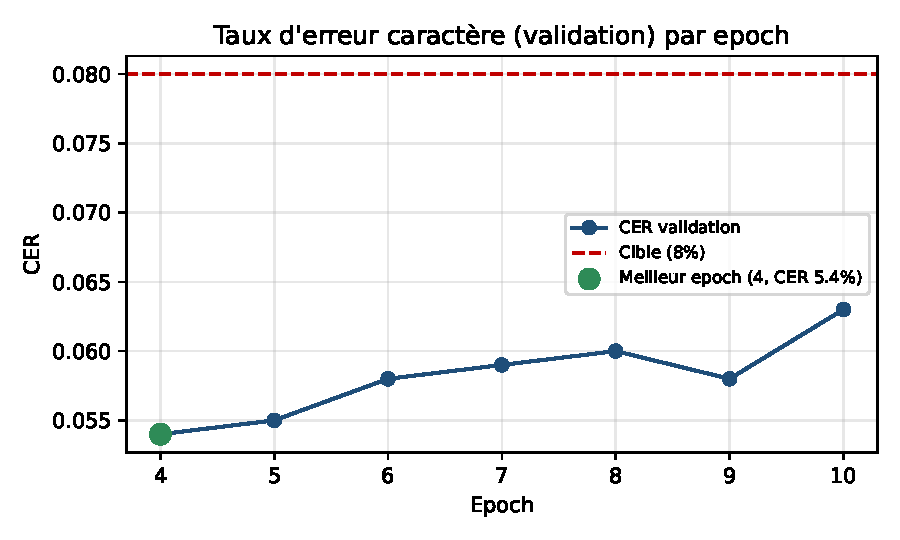
\includegraphics[width=\columnwidth]{figures/cer_par_epoch.pdf}
\caption{Taux d'erreur caractère (CER) de validation par epoch. La ligne
pointillée indique la cible de 8\,\%~; le point vert marque le meilleur epoch.}
\label{fig:cer}
\end{figure}

\begin{figure}[!t]
\centering
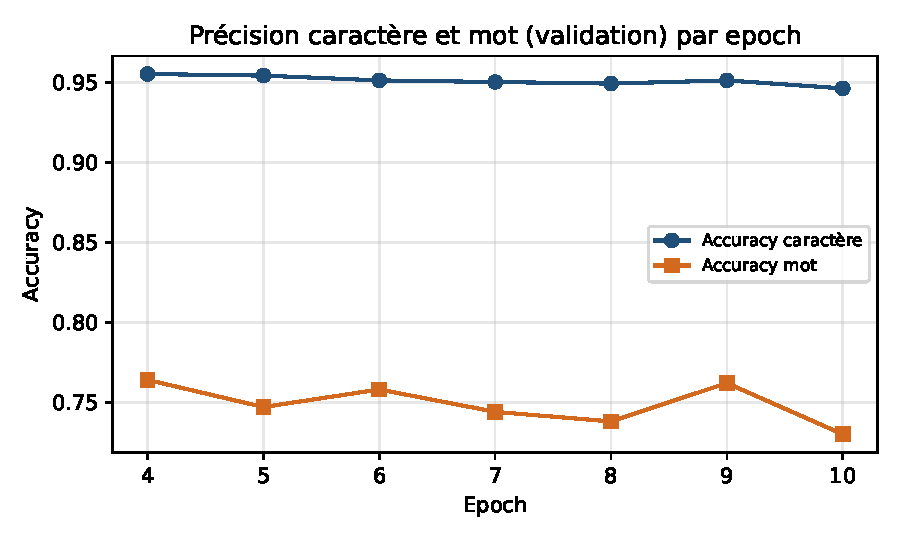
\includegraphics[width=\columnwidth]{figures/accuracy_par_epoch.pdf}
\caption{Précision caractère et précision mot (validation) par epoch.}
\label{fig:acc}
\end{figure}

\textbf{Validation qualitative.} Appliqué à une page complète de manuscrit
français (segmentation \textit{baseline} Kraken puis reconnaissance), le modèle
segmente et transcrit les lignes de texte gothique, illustrant l'enchaînement
segmentation~$\rightarrow$~reconnaissance du pipeline.

% ─────────────────────────────────────────────────────────────────
\section{Discussion et limites}
\textbf{Segmentation.} Le travail porte sur la \emph{reconnaissance} de lignes
pré-segmentées (fournies par CATMuS). L'évaluation d'un segmenteur de page (et la
métrique IoU associée) constitue une extension naturelle, réalisable sans
ré-entraînement du modèle de reconnaissance.

\textbf{Évaluation sur le test.} L'évaluation automatisée sur le \textit{test
set} via \texttt{ketos test} s'est heurtée à une incompatibilité de Kraken~7
avec les jeux binaires~; les métriques rapportées sont donc celles de
validation.

\textbf{Portée du transfert.} Les résultats valident le pipeline sur le français
médiéval. Le transfert vers l'écriture spéculaire de Léonard de Vinci reste
conditionné à la constitution d'une vérité terrain spécifique~: l'écriture en
miroir nécessite a minima un retournement horizontal des images, puis une phase
d'annotation.

% ─────────────────────────────────────────────────────────────────
\section{Conclusion et perspectives}
Nous avons construit un pipeline HTR reproductible et fine-tuné un modèle Kraken
sur le français du XIII\textsuperscript{e} siècle, atteignant un CER de
validation d'environ 4,5\,\%. Ce résultat valide la chaîne complète --- collecte,
préparation, fine-tuning, évaluation, visualisation --- et fournit une base
solide pour l'objectif initial.

Les prochaines étapes sont~: (i)~l'ajout d'un volet \emph{segmentation} avec
métrique IoU~; (ii)~une évaluation \textit{test} robuste~; (iii)~la constitution
progressive d'une vérité terrain pour les carnets de Léonard de Vinci
(retournement des images spéculaires, annotation assistée, puis fine-tuning du
présent modèle comme point de départ). À terme, le modèle pourrait transcrire
automatiquement des milliers de pages aujourd'hui difficilement accessibles,
ouvrant ce patrimoine aux historiens des sciences.

% ─────────────────────────────────────────────────────────────────
\section*{Disponibilité}
Code, configuration et tests sont disponibles dans le dépôt du projet. Les
figures sont générées automatiquement depuis les métriques d'entraînement
(\texttt{paper/make\_figures.py}).

\begin{thebibliography}{9}
\bibitem{kraken} B.~Kiessling, \textit{Kraken --- an universal text recognizer
for the humanities}, Digital Humanities, 2019.
\bibitem{catmus} S.~Torres Aguilar \textit{et al.}, \textit{CATMuS Medieval: A
multilingual large-scale cross-century dataset in Latin script for HTR}, 2024.
\bibitem{ctc} A.~Graves \textit{et al.}, \textit{Connectionist Temporal
Classification}, ICML, 2006.
\end{thebibliography}

\end{document}
